\subsection{Estado de resultados}

El estado de resultados se proyecta a cinco años, permitiendo analizar detalladamente los flujos de dinero en la empresa y considerando los costos involucrados para obtener las utilidades netas de cada año fiscal.

En la tabla \ref{estado} se presenta la utilidad bruta, obtenida al deducir los costos de ventas de las ventas netas. También se muestra la utilidad operacional, calculada restando los gastos administrativos de la utilidad bruta. Finalmente, se incluyen los gastos financieros y pre-operativos, que permiten determinar la utilidad antes de impuestos, considerando la tasa de impuesto sobre la renta aplicable al año gravable 2025.

\vspace{2mm}
\begin{minipage}{0.9\textwidth}
\centering
\captionof{table}[{Estado de resultados }]{ Estado de resultados }
\label{estado}
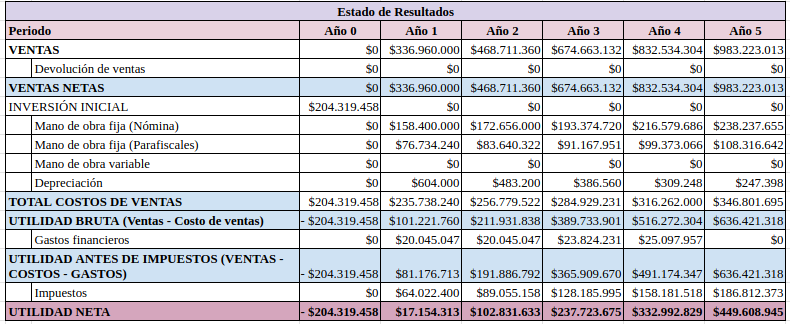
\includegraphics[width=0.9\textwidth]{Content/Images/AF/EstadoDeResultados.png}
\footnote{Nota. \textup{Fuente : Autores}}
\end{minipage}
\newpage